\sloppy \section{Memoria} \label{sec:richiami_memoria}
Il collo di bottiglia principale per le prestazioni di un calcolatore è sicuramente costituito dalla memoria. Distinguiamo DRAM (Dynamic Random  Access Memory), poco costose ma lente e SRAM (Static Random Access Memory), molto più costose a causa dell'elevato numero di transistori ma molto veloci. Viste le differenze di costo e di velocità, diventa conveniente costruire una gerarchia di livelli di memoria, con la memoria più veloce posta più vicino al processore e quella più lenta, meno costosa, posta più distante.
Sfruttando il \textbf{principio di località}, l’architettura della memoria in un calcolatore moderno viene implementata come una \textit{gerarchia multilivello}, costituita da un insieme di memorie caratterizzate da differenti \textbf{tempi di accesso}, \textbf{capacità} e \textbf{costo per bit}. A parità di capacità, le memorie con prestazioni più elevate risultano sensibilmente più costose rispetto a quelle più lente; di conseguenza, esse vengono realizzate con dimensioni ridotte e collocate nei livelli più alti della gerarchia, ossia in prossimità della \textbf{CPU}. Al contrario, le memorie di capacità maggiore, ma con latenze più elevate e costo per bit inferiore, sono collocate nei livelli più bassi, fungendo da \textit{storage} di supporto.  

L'obiettivo principale di tale organizzazione è quello di fornire al programmatore l'illusione di disporre di un’unica memoria avente contemporaneamente la \textbf{velocità} tipica dei livelli più alti (ad esempio le \textit{cache}) e la \textbf{capacità} tipica dei livelli più bassi (come la \textit{memoria principale} e la \textit{memoria secondaria}). In tal modo, la gerarchia di memoria realizza un compromesso efficace tra \textit{prestazioni}, \textit{costo} e \textit{scalabilità}, nascondendo la complessità dell’accesso ai diversi livelli e ottimizzando l’utilizzo delle risorse hardware disponibili.
Tecnicamente, il livello più elevato della gerarchia di memoria dovrebbe essere identificato con il \textbf{register file} interno alla \textbf{CPU}. Tuttavia, la sua gestione risulta peculiare ed estremamente semplificata, poiché la maggior parte delle problematiche legate al suo utilizzo viene affrontata direttamente dal \textbf{compilatore}. Per tale motivo, esso non verrà considerato nell'analisi seguente. L'attenzione sarà invece rivolta ai livelli immediatamente successivi, ovvero alle cosiddette \textit{memorie cache}, che costituiscono le gerarchie più alte della \textit{memoria di lavoro}.  

\noindent
Nei calcolatori moderni è sempre presente almeno un livello di \textbf{cache}, e molto spesso ne sono disponibili due o più, organizzati gerarchicamente come \textbf{L1}, \textbf{L2} e, in alcuni casi, \textbf{L3}. La cache è strutturata in unità dette \textit{blocchi} o \textit{linee di cache} (\textit{cache lines}), che rappresentano la minima quantità di informazione trasferibile fra due livelli adiacenti della gerarchia.  

\noindent
Quando la CPU richiede un dato e questo risulta già contenuto in uno dei blocchi presenti nella cache di livello superiore, si verifica un \textbf{cache hit}, ossia un accesso corretto ed immediato ai dati richiesti. Al contrario, se il dato non è disponibile nella cache, si verifica un \textbf{cache miss}; in tal caso è necessario accedere al livello inferiore della gerarchia, individuare il blocco che contiene il dato richiesto e trasferirlo nel livello superiore, aggiornando la cache. Questo meccanismo consente di ridurre in maniera significativa la latenza media di accesso alla memoria, pur introducendo problematiche di \textit{gestione della sostituzione dei blocchi} e di \textit{politiche di coerenza}, che rappresentano aspetti cruciali nell'architettura delle memorie moderne.

\subsection{Problema del piazzamento di un blocco}
Consideriamo innanzitutto il problema del \textbf{piazzamento di un blocco} nella memoria cache. Durante l'esecuzione di un programma, la \textbf{CPU} può tentare di accedere, in linea di principio, a qualunque parola all'interno dello \textit{spazio totale di indirizzamento}. Tale spazio può essere idealmente assimilato all'intera \textbf{memoria RAM}, che rappresenta il livello più basso della gerarchia di memoria di lavoro. Tuttavia, la capacità della cache è di gran lunga inferiore rispetto a quella della memoria principale; ne consegue che non è possibile mantenere simultaneamente in cache tutte le parole potenzialmente indirizzabili.  
Diventa quindi necessario stabilire un meccanismo che definisca come ciascuna parola della memoria indirizzabile possa essere, quando richiesto, mappata in una specifica posizione della cache. In altri termini, occorre definire una \textbf{corrispondenza} tra l'\textit{indirizzo di memoria} di una parola e la \textit{locazione cache} che potrà contenerla.  
A questo scopo, l'architettura dei sistemi di memoria ha introdotto tre principali modalità di organizzazione:  

\begin{itemize}
  \item \textbf{Cache a indirizzamento diretto}: ogni blocco di memoria principale può essere memorizzato in una sola posizione predeterminata della cache, stabilita in base a una funzione di mappatura (tipicamente, una parte dell'indirizzo). Questa soluzione è semplice ed efficiente in termini di hardware, ma può portare a numerosi \textit{conflict miss} quando più blocchi competono per la stessa posizione.
  
  \item \textbf{Cache set-associativa a $n$ vie}: la cache è suddivisa in insiemi (\textit{sets}), ciascuno composto da $n$ linee. Un blocco può essere memorizzato in qualunque linea del set corrispondente. Questa soluzione rappresenta un compromesso tra flessibilità e complessità hardware, riducendo sensibilmente i conflitti rispetto al caso diretto.
  
  \item \textbf{Cache completamente associativa}: un blocco può essere collocato in qualunque posizione della cache, senza vincoli. Questo approccio minimizza i \textit{miss da conflitto}, ma richiede circuiteria di ricerca più complessa e costosa, in quanto ogni accesso implica il confronto parallelo dell'indirizzo con tutte le linee della cache.
\end{itemize}
\noindent
Ciascuna di queste soluzioni presenta vantaggi e svantaggi in termini di \textbf{latenza di accesso}, \textbf{costo hardware} e \textbf{frequenza dei miss}, rendendo la scelta del tipo di mappatura un elemento cruciale nella progettazione delle architetture di memoria.
% \begin{figure}[ht]
%     \centering
%     \setlength{\fboxrule}{0.5pt} % spessore sottile
%     \setlength{\fboxsep}{0pt}    % senza spazio interno
%     \fbox{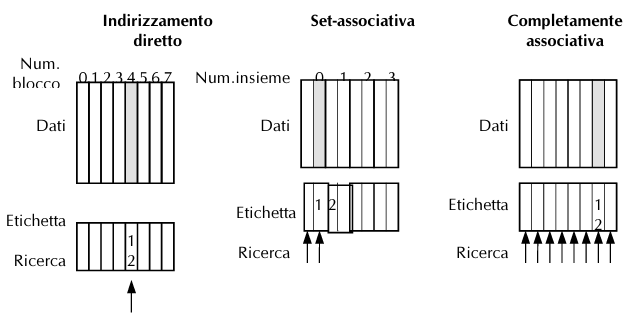
\includegraphics[width=0.6\textwidth]{fig/chapter_1/gerarchie_memoria.png}}
% \end{figure}


\noindent Nel caso di \textbf{cache a indirizzamento diretto} ogni locazione di memoria corrisponde esattamente ad una locazione nella cache. Chiamando $I_c$ l'indirizzo del blocco nella cache, $I_m$ l'indirizzo del blocco in memoria e $N$ il numero di blocchi contenuti dalla cache la corrispondenza è data da:

\begin{equation}
    I_c = I_m \ \bmod \ n 
\end{equation}

Poichè il numero degli elementi della cache è una potenza di 2, l'operazione modulo può essere fatta considerando i $\log_2N$ bit meno significativi, che sono usati come indice della cache.  

\begin{figure}[ht]
    \centering
    \setlength{\fboxrule}{0.5pt} % spessore sottile
    \setlength{\fboxsep}{0pt}    % senza spazio interno
    \fbox{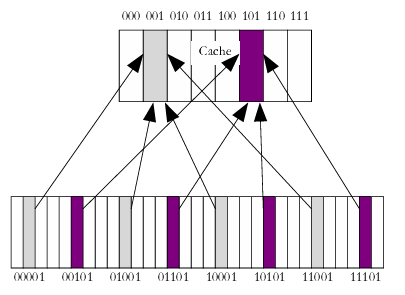
\includegraphics[width=0.6\textwidth]{fig/chapter_1/direct_mapping.png}}
\end{figure}

\noindent Nel caso di \textbf{cache completamente associativa}, ogni blocco di memoria principale può essere collocato in una qualunque posizione della memoria cache, senza vincoli deterministici sul piazzamento. La corrispondenza tra un indirizzo di memoria in \textbf{RAM} e una locazione della cache non è quindi stabilita a priori, ma viene gestita mediante la ricerca del blocco desiderato all'interno dell'intera cache.  
Poiché un blocco può risiedere in qualunque posizione, al momento dell'accesso è necessario confrontare l'\textit{indirizzo} richiesto dalla CPU con tutti gli identificativi (i cosiddetti \textbf{tag}) dei blocchi memorizzati in cache. Questo richiede la presenza di un meccanismo hardware di confronto parallelo (\textit{associative search}), che rende la soluzione estremamente flessibile ma costosa dal punto di vista circuitale.  

\noindent
Una \textbf{cache set-associativa a $n$ vie} è organizzata in un numero finito di \textbf{insiemi} (\textit{sets}), ciascuno dei quali contiene $n$ linee o blocchi. La memoria principale (\textbf{RAM}) è anch'essa concettualmente suddivisa in blocchi; ciascun blocco della RAM viene mappato in modo deterministico su un solo insieme della cache, ma all'interno di tale insieme può essere collocato in una qualunque delle $n$ vie disponibili.  

\noindent
In termini formali, l'indice dell'insieme si ottiene mediante l'operazione:  

\[
(\text{Indirizzo blocco})_{set} = (\text{Indirizzo blocco})_{mem} \ \bmod \ (\# \text{insiemi})
\]

\noindent
dove il numero degli insiemi è pari al rapporto tra il numero totale di linee della cache e il numero di vie $n$.  

\medskip
\noindent
\textbf{Esempio d’uso:}  
Si consideri una cache composta da 64 linee, organizzata come \textbf{4-vie set-associativa} (\(n=4\)). In questo caso:  

\[
\# \text{insiemi} = \frac{64}{4} = 16
\]

\noindent
Sono quindi necessari \(\log_2 16 = 4\) bit dell'indirizzo per individuare l'insieme.  
Supponiamo che la CPU richieda il blocco di memoria con indirizzo decimale \(45\). L'indice dell'insieme risulta:  

\[
45 \bmod 16 = 13
\]

\noindent
Pertanto, il blocco 45 può essere collocato in qualunque delle 4 vie appartenenti all'insieme 13.  
Se in seguito la CPU richiede il blocco con indirizzo 61, avremo:  

\[
61 \bmod 16 = 13
\]

\noindent Anche questo blocco si mapperà nello stesso insieme 13, potendo occupare una delle 4 vie disponibili. Se tutte le vie dell'insieme risultassero già occupate, uno dei blocchi dovrebbe essere sostituito secondo una \textit{politica di rimpiazzo}.

\noindent
Questo schema rappresenta un \textit{compromesso intermedio} tra la cache a indirizzamento diretto (che vincola rigidamente la posizione) e quella completamente associativa (che lascia piena libertà di collocamento). In una cache set-associativa, la mappatura dal blocco RAM all'insieme avviene tramite indirizzamento diretto, mentre la ricerca del blocco avviene confrontando i \textbf{tag} di tutte le vie dell'insieme selezionato.

\begin{figure}[ht]
    \centering
    \setlength{\fboxrule}{0.5pt} % spessore sottile
    \setlength{\fboxsep}{0pt}    % senza spazio interno
    \fbox{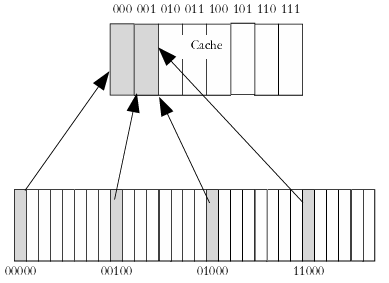
\includegraphics[width=0.6\textwidth]{fig/chapter_1/associative_n_vie.png}}
\end{figure}

Ogni politica di piazzamento può in realtà essere considerata una variazione di quella set
associativa: una cache a indirizzamento diretto è una cache set-associativa a 1 vie, in cui ogni elemento della cache contiene un blocco e forma un insieme di un solo elemento. Una cache di m elementi completamente associativa è una cache set-associativa a m vie: c'è un
solo insieme di m blocchi e un elemento può trovarsi in uno qualsiasi dei blocchi dell'insieme.

\subsection{Problema della ricerca di un blocco}
Poiché ogni linea della cache può contenere blocchi provenienti da differenti locazioni della \textbf{memoria principale}, è necessario disporre di un meccanismo che consenta di stabilire se il dato richiesto dalla CPU sia effettivamente presente nella cache. A tale scopo, ad ogni elemento della cache viene associato un insieme di \textbf{etichette} (\textit{tag}), che contengono le informazioni necessarie per identificare la corrispondenza tra l'indirizzo richiesto e quello del blocco memorizzato nella linea.  

In altre parole, durante un accesso, l'indice della cache individua una o più linee candidate (a seconda della politica di piazzamento: indirizzamento diretto, set-associativa o completamente associativa), e i tag vengono confrontati con la parte più significativa dell'indirizzo in memoria. Solo in caso di uguaglianza tra il tag memorizzato e quello dell'indirizzo richiesto si verifica un \textbf{cache hit}; in caso contrario si ha un \textbf{cache miss}.  

Un'ulteriore informazione fondamentale è il \textbf{bit di validità} (\textit{validity bit}), che indica se la linea della cache contiene dati effettivamente validi. Infatti, al momento dell'accensione del processore, la cache risulta inizialmente vuota, e le etichette non hanno alcun significato: tutte le linee vengono quindi marcate come \textit{non valide}. Il bit di validità è del tutto indipendente dalla filosofia di piazzamento scelta ed è quindi presente in qualsiasi schema di organizzazione della cache.  


\noindent A titolo esemplificativo, consideriamo una cache a indirizzamento diretto da 4 Kbyte, blocco corrispondente ad una sola parola di 32 bit; Questa situazione viene schematizzata come illustrato nella seguente figura.

\begin{figure}[ht]
    \centering
    \setlength{\fboxrule}{0.5pt} % spessore sottile
    \setlength{\fboxsep}{0pt}    % senza spazio interno
    \fbox{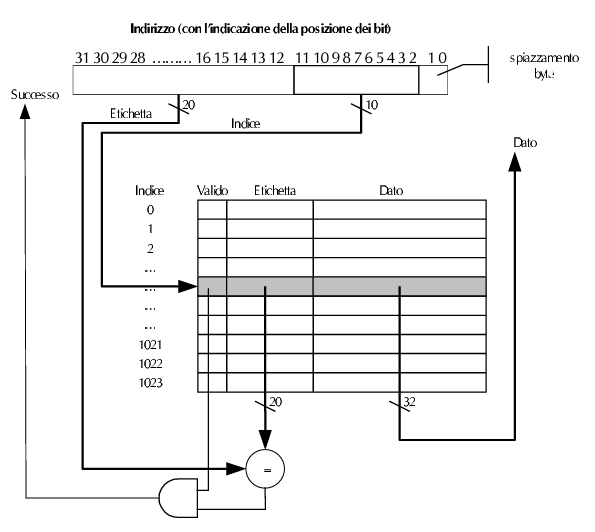
\includegraphics[width=0.6\textwidth]{fig/chapter_1/schema_4_kb.png}}
\end{figure}

\noindent Lo schema descritto finora non sfrutta il principio di località spaziale, in quanto ogni parola corrisponde ad un blocco. Per trarre vantaggio dalla località spaziale è necessario che la dimensione del blocco della cache sia maggiore della dimensione della parola in memoria, in modo che il blocco contenga più di una parola. Serve quindi un nuovo campo in cui suddividere l'indirizzo che corrisponda allo spiazzamento della parola nel blocco. In caso di \textit{miss}, dalla memoria centrale vengono prelevate più parole adiacenti che hanno un elevata probabilità di essere richiesta a breve. Il numero totale di etichette è inferiore in questo caso, perchè ogni etichetta è utilizzata per più parole. 

\noindent Consderiamo il caso più interessante della ricerca di un blocco in una cache associativa a n vie.
Ogni blocco della cache comprende ancora un'etichetta che permette di individuare l'indirizzo del blocco in memoria principale. Il valore dell'indice serve a selesionare l'insieme che contiene l'indirizzo desiderato. Se la CPU produce una richiesta ad un determinato indirizzo, viene selezionato un gruppo di blocchi corrispondenti all'insieme specificato, e ne vengono controllate \textit{in parallelo} le etichette. 
Vediamo a titolo di esempio lo schema generale di una cache set-associativa a 4 vie da 4 Kbye e blocco da 32 bit:

\begin{figure}[ht]
    \centering
    \setlength{\fboxrule}{0.5pt} % spessore sottile
    \setlength{\fboxsep}{0pt}    % senza spazio interno
    \fbox{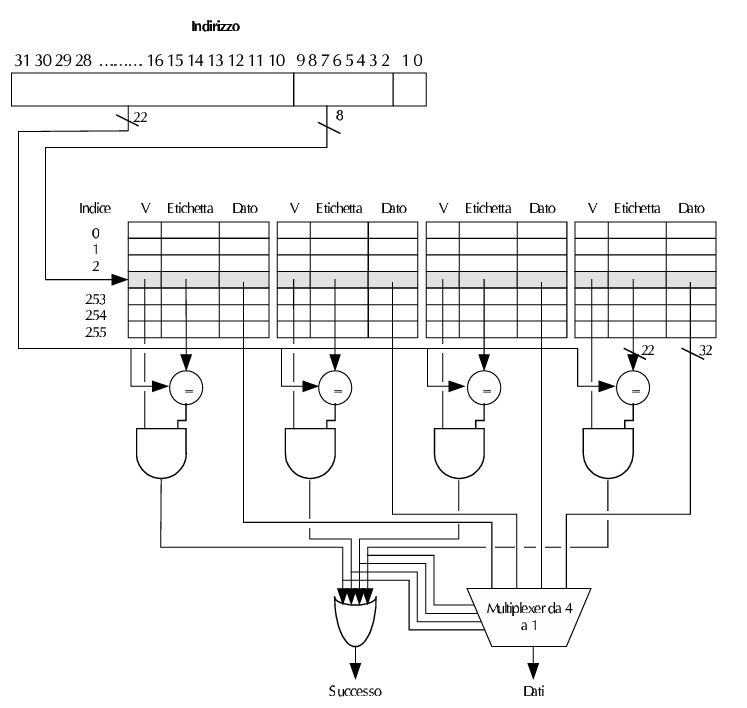
\includegraphics[width=0.6\textwidth]{fig/chapter_1/set_associative_scheme.png}}
\end{figure}

Se si mantiene costante la dimensione totale, al crescere dell'associatività aumenta anche il
numero dei blocchi compresi nell'insieme, e questo corrisponde al numero dei confronti  associativi che devono essere effettuati per realizzare una ricerca in parallelo. Ogni volta che si raddoppia il grado di associatività si raddoppia il numero di blocchi compresi in un insieme e si  dimezza il numero degli insiemi. Al tempo stesso, ogni incremento dell'associatività di un fattore due fa diminuire di un bit la dimensione dell'indice e aumentare di un bit la dimensione dell'etichetta. Vale la pena osservare che aumentando l'associatività aumenta il numero dei comparatori e aumenta anche la dimensione di ogni singolo comparatore, e ciò corrisponde ad una maggiore complessità circuitale. In una cache completamente associativa c'è un unico insieme e tutti i blocchi devono essere esaminati in parallelo: di conseguenz l'intero indirizzo, a parte lo spiazzamento nel blocco, viene confrontato con l'etichetta di ogni blocco: occorrono quindi tanti comparatori quanti sono i blocchi. (Dualmente, in una cache a indirizzamento diretto è necessario un solo comparatore, dato che l'elemento può essere in una sola posizione).

\noindent In una cache set-associativa a n vie, sono necessari n comparatori, oltre a un multiplexer da n a 1 per scegliere tra gli n possibili blocchi dell'insieme selezionato. I comparatori individuano quale elemento dell'insieme corrisponde all'etichetta e forniscono quindi gli ingressi di selezione del multiplexer, in modo da avviare all'uscita uno solo degli n blocchi dell'insieme selezionato.
L'accesso alla cache si effettua utilizzando l'indice per individuare l'insieme e poi esaminando in parallelo tutti gli n blocchi dell'insieme.
Oltre al costo correlato ai comparatori aggiunti occorre tenere conto dei ritardi imposti dalla necessità di confrontare e selezionare l'elemento desiderato tra quelli dell'insieme. D'altronde, è chiaro che la soluzione completamente associativa permette uno sfruttamento migliore dello spazio disponibile in cache, dato che, ad esempio, in fase di scrittura, è possibile trasferire un blocco dalla RAM a un qualsiasi blocco della cache. In ogni
gerarchia di memoria, la scelta tra lo schema a indirizzamento diretto, quello set-associativo e quello completamente associativo dipende dal confronto tra il costo di un fallimento e quello di realizzazione dell'associatività, sia dal punto di vista del tempo sia da quello della circuiteria aggiuntiva.

\subsection{Problema della sostituzione di un blocco}
Si consideri ora il problema della \textbf{sostituzione di un blocco} nella cache. Quando si verifica un \textit{cache miss}, è necessario decidere quale linea della cache liberare per fare spazio al nuovo blocco proveniente dalla memoria principale.  

Nel caso di una \textbf{cache a indirizzamento diretto}, il problema non si pone: l'indirizzo di memoria individua un'unica linea di cache e il blocco presente in quella posizione viene automaticamente rimpiazzato. Al contrario, in una \textbf{cache completamente associativa}, ogni blocco della cache è un potenziale candidato per la sostituzione, e diventa quindi necessario adottare una \textit{politica di rimpiazzo}. Nelle \textbf{cache set-associative}, l'insieme di appartenenza del blocco è determinato in maniera univoca dall'indirizzo, ma la scelta deve comunque essere effettuata tra le $n$ vie appartenenti all'insieme selezionato.  

Le principali strategie di sostituzione comunemente adottate sono tre:  

\begin{itemize}
  \item \textbf{Sostituzione casuale (Random)}: la linea da rimpiazzare viene scelta in maniera casuale tra le candidate. Tale metodo è semplice da implementare, eventualmente con l'ausilio di componenti hardware per la generazione pseudo-casuale, ma non garantisce prestazioni ottimali.
  
  \item \textbf{Least Recently Used (LRU)}: viene sostituito il blocco che non è stato utilizzato da più tempo. Una possibile implementazione elementare associa ad ogni blocco un contatore: quando un blocco viene caricato, il contatore viene inizializzato al valore massimo; ad ogni accesso a un blocco diverso, i contatori vengono decrementati. Al momento della sostituzione, viene scelto il blocco con contatore minimo. Sebbene LRU sia molto efficace nel ridurre i \textit{miss}, la sua implementazione hardware può risultare costosa nelle cache di grandi dimensioni.
  
  \item \textbf{First In First Out (FIFO)}: viene sostituito il blocco caricato da più tempo, indipendentemente dal suo utilizzo negli accessi recenti. Questo schema è semplice da implementare mediante una coda circolare, ma può risultare meno performante rispetto a LRU in presenza di dati con elevata riutilizzabilità.
\end{itemize}

\subsection{Problema della strategia di scrittura}
Infine, consideriamo il problema della \textbf{strategia di scrittura}. Esso nasce dal fatto che, quando il processore deve memorizzare il risultato di un'operazione, è desiderabile che l'istruzione di scrittura venga eseguita con la massima velocità possibile (quindi accedendo alla \textbf{cache}), ma al tempo stesso è necessario che i dati contenuti nella cache siano \textbf{coerenti} con quelli presenti nella memoria principale.  

\noindent
Le principali strategie adottate sono due: \textbf{write-through} e \textbf{write-back}.  
Nell'approccio \textbf{write-through}, ogni operazione di scrittura aggiorna simultaneamente sia il blocco presente nella cache sia quello corrispondente in memoria principale. In questo modo la coerenza è sempre garantita, ma al prezzo di un tempo di scrittura maggiore, poiché ogni operazione implica un accesso anche alla memoria più lenta.  

\noindent
Nell’approccio \textbf{write-back} (o \textit{copy-back}), invece, i dati vengono scritti inizialmente solo nella cache. La copia nel livello inferiore della gerarchia avviene soltanto quando il blocco modificato deve essere sostituito. Di conseguenza, dopo un'operazione di scrittura, la cache può contenere valori diversi rispetto alla RAM. In questo caso si parla di \textbf{incoerenza}: il blocco può essere \textit{clean} (non modificato) oppure \textit{dirty} (modificato). Per gestire questa condizione, ogni linea della cache è dotata di un \textbf{dirty bit}, che segnala se il contenuto è stato modificato rispetto alla memoria principale.  

\noindent
Poiché le prestazioni delle CPU crescono a un ritmo molto più elevato rispetto a quelle delle memorie DRAM, la frequenza delle scritture generate dal processore tende a superare quella sostenibile dalla memoria principale. Inoltre, secondo il \textbf{principio di località}, se un blocco viene scritto una volta, è altamente probabile che venga riscritto più volte prima di essere sostituito. Per questi motivi, la strategia \textit{write-back} è destinata a diventare sempre più diffusa nei sistemi moderni. Entrambe le soluzioni presentano vantaggi e svantaggi.  

\noindent
I principali \textbf{vantaggi della write-back} sono:  
\begin{itemize}
  \item le singole parole possono essere scritte alla frequenza accettata dalla cache, senza attendere i tempi della memoria principale;  
  \item più scritture all'interno dello stesso blocco richiedono una sola operazione di scrittura nel livello inferiore al momento della sostituzione;  
  \item quando i blocchi vengono trasferiti, l'uso di un bus ampio permette di sfruttare la scrittura a livello di intero blocco, migliorando anche la gestione dei fallimenti in lettura.  
\end{itemize}

\noindent
I principali \textbf{vantaggi della write-through} sono invece:  
\begin{itemize}
  \item i fallimenti in lettura risultano meno costosi, poiché non richiedono mai la scrittura preventiva di un blocco nel livello inferiore (al contrario, con write-back un blocco \textit{dirty} deve essere scritto prima di essere sostituito);  
  \item lo schema è più semplice da implementare rispetto al write-back; tuttavia, per essere efficace in un sistema ad alte prestazioni, una cache \textit{write-through} deve essere dotata di un \textbf{write buffer}, così da non costringere la CPU ad attendere i tempi di accesso della memoria principale.  
\end{itemize}
